\chapter{Proposta de Algoritmo}
\label{algorithm-proposition}

Neste capítulo será apresentado o algoritmo que este trabalho visa propor, detalhes de seu funcionamento e suas vantagens.

\section{Motivação}
\label{motivation}

A evolução no campo da criptografia é constante e há sempre novas propostas de algoritmos que focam em solucionar um obstáculo imposto por possíveis atacantes e seus métodos para se obter informações sigilosas.

O algoritmo proposto neste trabalho visa diminuir as possibilidades de análises de frequência de um texto cifrado. É uma nova modalidade na produção de texto cifrado utilizando cifra de fluxo. 


\section{Funcionamento}
\label{functioning}

O algoritmo de cifração terá como entrada um texto em claro e uma sequência de números pseudo-aleatórios e terá como objetivo produzir um texto cifrado onde as frequências de ocorrência dos valores de \textit{bytes} cifrados seja totalmente balanceada.

O mecanismo utilizado para este balanceamento será produzir o texto cifrado em “rodadas” de 256 \textit{bytes} em que cada valor de \textit{byte} cifrado só aparece uma vez por rodada. Isto é, os 256  \textit{bytes} cifrados de cada rodada são distintos, porém a ordem em que aparecem em cada rodada é aleatória (ou melhor dizendo, pseudo-aleatória).

Para se garantir que nenhum valor de \textit{byte} cifrado se repita em uma rodada, utiliza-se uma tabela de 256 posições. No início da rodada a tabela tem todas a suas 256 posições marcadas como não ocupadas. Para cada \textit{byte} de texto em claro que se deseja cifrar será feito um ou-exclusivo com o valor correspondente fornecido pelo gerador de números aleatórios resultando no \textit{byte} pré-cifrado. Tendo-se obtido o \textit{byte} pré-cifrado verifica-se se este valor já está ocupado na tabela. 

\begin{figure}[h]
	\centering
	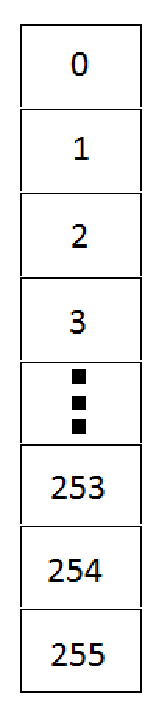
\includegraphics[scale=0.5]{figuras/tabela.eps}
	\caption{Tabela de \textit{byte} para uso do algoritmo}
\end{figure}

Caso o valor do \textit{byte} pré-cifrado obtido corresponda a uma posição já ocupada na tabela,temos um conflito. Este valor não será aceito como \textit{byte} cifrado e o próximo valor da sequência pseudo-aleatória será utilizado para tentar novamente a cifração do \textit{byte} em claro. Este procedimento será repetido até que o valor pré-cifrado obtido corresponda a uma posição não ocupada na tabela, quando então este valor será aceito como o \textit{byte} cifrado (correspondente ao byte de texto em claro que está sendo processado pelo cifrador). O número de valores da sequência pseudo-aleatória não utilizados será contabilizado em uma variável j. 

Caso o valor do \textit{byte} pré-cifrado obtido corresponda a uma posição não ocupada na tabela, este valor será aceito como \textit{byte} cifrado, a posição correspondente na tabela será marcada como ocupada, e a variável j será reinicializada com o valor 0.

Aqui se introduz o problema de como enviar ao decifrador as seguintes informações:

\begin{enumerate}
	\item Que houve um conflito na cifração ( quando o mesmo ocorrer)
	\item Em ocorrendo o conflito, qual o número de valores na sequência pseudo-aleatória deverão ser desprezados na decifração.
\end{enumerate}


\begin{figure}[h]
	\centering
	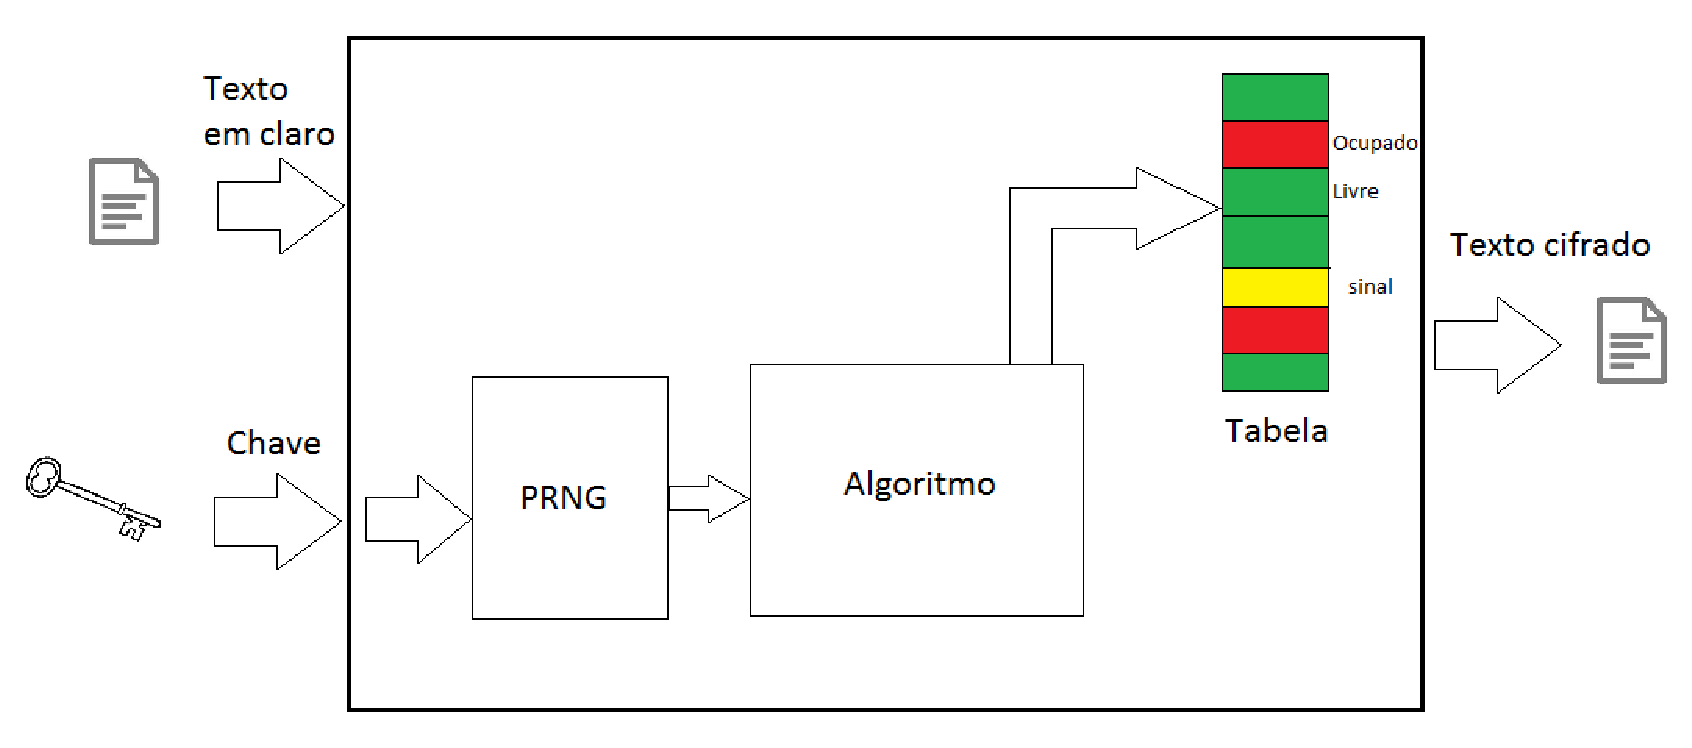
\includegraphics[scale=0.4]{figuras/funcionamento.eps}
	\caption{Esquema do algoritmo de cifração}
\end{figure}

Para informar ao decifrador que houve um conflito na cifração propomos a utilização de um valor de \textit{byte} entre 0 e 255 chamado de \textbf{sinal}.Este valor é o primeiro \textit{byte} do gerador de \textit{bytes}, e será atualizado a cada vez que a tabela se completa, se tornando o primeiro valor do gerador pseudo-aleatório da próxima rodada. Este valor será enviado pelo cifrador como parte da sequência de \textit{bytes} cifrados indicando ao decifrador que o \textit{byte} seguinte na sequência de \textit{bytes} cifrados corresponderá ao número de valores da sequência produzida pelo gerador pseudo-aleatório que deverão ser desprezados. O decifrador saberá o \textit{byte} recebido é sinal por meio de um contador, que será incrementado a cada vez que um \textit{byte} for decifrado. Após o envio do \textit{byte} de sinal, o cifrador  enviará o valor da variável j (também cifrado), e finalmente enviará o \textit{byte} cifrado.

O processo de cifração, que pode ser visto no pseudo-código \ref{pseudo-codigo}, segue os seguintes caminhos:

%\begin{figure}[h]
%	\centering
%	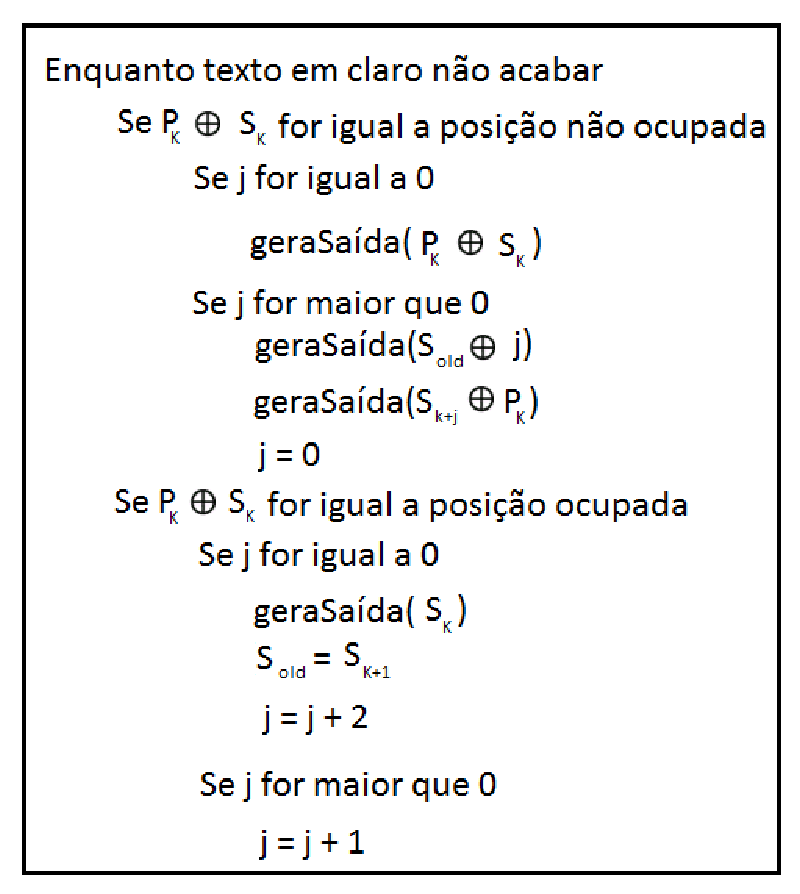
\includegraphics[scale=0.6]{figuras/pseudocondigo.eps}
%	\caption{Pseudo código do algoritmo de cifração}
%	\label{pseudo-codigo}
%\end{figure}

O caminho ideal é o que o resultado da operação ou-exclusivo entre o \textit{byte} do texto em claro e o número aleatório correspondente sempre corresponda a uma posição livre na tabela de balanceamento.

\begin{lstlisting}[caption={Pseudo-Código Cifração}, label=pseudo-codigo]
signal = S[0] // primeiro sinal do gerador
table[255] = '0'
count = 0;
while(plainText != EOF)
	if(table[plainText[k] ^ S[k]] != '1'){
		if(j == 0)
			output(plainText[k] ^ S[k]);
		if( j > 0){
			output(S[old] ^ j);
			output(S[k+j] ^ plainText[k]);
			j = 0;
		}
		count++;
	}
	if(tabela[plainText[k] ^ S[k] == '1'){
		if(j == 0){
			output(signal);
			S[old] = S[k+1];
			j = 1;		
		}
		if(j > 0){
			j = j + 1;
		}
	}
	//se tabela completar
	if(count == 256){
		resetTable();
		signal = S[k]
		count = 0;
	}
}
    \end{lstlisting}


Caso se detecte um conflito de resultados na tabela de balanceamento, é enviado o \textit{byte} de sinal para o receptor da mensagem, pois com isso o receptor saberá que o próximo valor recebido será a quantidade de números pseudo-aleatórios que deverão ser descartados da sequência. 

Então o algoritmo vai executar o comando de descartar os números pseudo-aleatórios, até que se encontre um resultado em uma posição que esteja livre na tabela de balanceamento. 


\begin{figure}[h]
	\centering
	\includegraphics[scale=0.4]{figuras/metodo_de_decifra.eps}
	\caption{Esquema do algoritmo de decifração}
\end{figure}

Ao encontrar essa posição livre, o algoritmo (no lado da cifração) enviará o \textit{byte} de sinal (sem cifrar) e em seguida enviará o resultado do ou-exclusivo entre \textbf{j} (quantidade de números descartados) e S$_{old}$. Então o valor de \textbf{j} é novamente reinicializado como 0.

Quando a tabela for totalmente concluída, a rodada termina e o processo se inicia de novo com uma nova rodada, reinicializando-se a tabela (todas as suas posições são marcadas como desocupadas) e um novo sinal é gerado. Esse processo termina quando os \textit{bytes} do texto em claro forem todos cifrados. A cada rodada o \textit{byte} de sinal terá um valor diferente. Escolhemos o primeiro \textit{byte} da sequência de números pseudo-aleatórios da rodada como o \textit{byte} de sinal.

Podemos observar o processo de decifração no pseudo-código \ref{pseudo-codigo-decifrar}. Neste não é necessário se utilizar a tabela de balanceamento. Para se realizar a decifração é necessário que o decifrador tenha a capacidade de produzir a mesma sequência de números aleatórios que o cifrador. Isto implica que ele deve ter a mesma chave que foi utilizada no processo de cifrar.

No início de cada rodada na decifração, o primeiro \textit{byte} da sequência aleatória é separado como o \textit{byte} de sinal. Os valores pseudo-aleatórios seguintes serão usados no processo de decifração. O primeiro passo no processo de decifração é comparar o \textit{byte} cifrado recebido com o valor de sinal utilizado na rodada. 


%\begin{figure}[h]
%	\centering
%	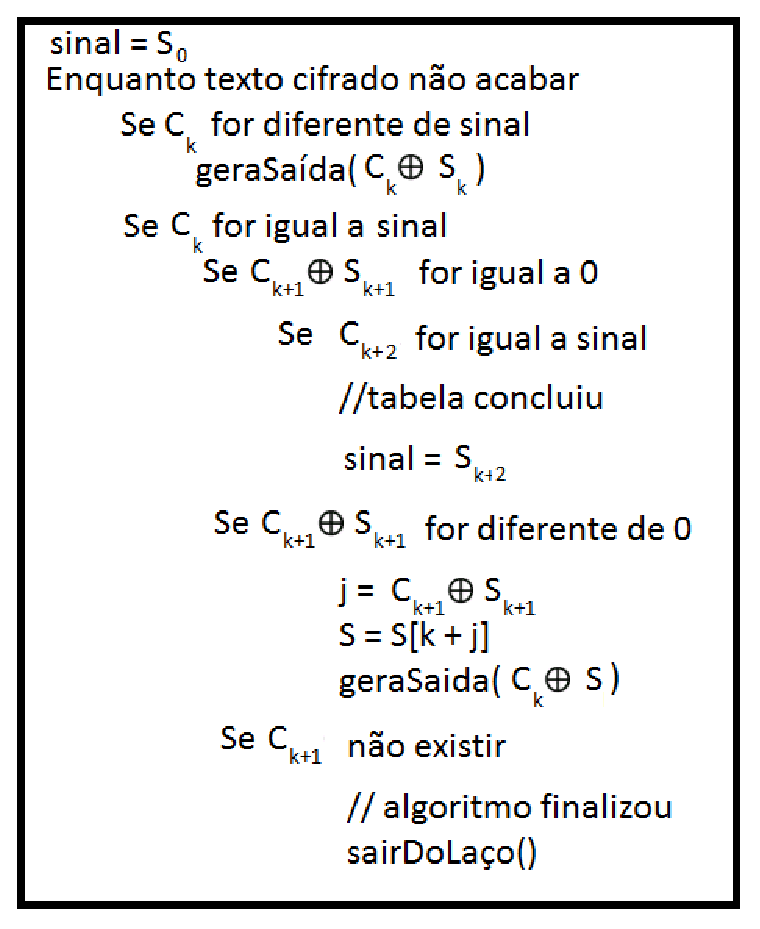
\includegraphics[scale=0.7]{figuras/funcionamento_Decifra.eps}
%	\caption{Pseudo código do algoritmo de decifração}
%	\label{pseudo-codigo-decifrar}
%\end{figure}

    \begin{lstlisting}[caption={Pseudo-Código Decifração}, label=pseudo-codigo-decifrar]
signal = S[0] // primeiro sinal do gerador
count = 0;
while(cipherText != EOF)
	if(C[k] != sinal){
		output(C[k] ^ S[k];
		count++;
	}
	if((C[k] == signal){
		j = C[k+1] ^ S[k+1];
		S = S[k+j];
		output(C[k] ^ S);
		count++;
	}
	//se tabela completar
	if(count == 256){
		resetTable();
		signal = S[k]
		count = 0;
	}
}
    \end{lstlisting}

Se o valor do \textit{byte} cifrado for diferente do valor do sinal utilizado na rodada, realiza-se a operação ou-exclusivo entre o \textit{byte} cifrado e o valor fornecido pelo gerador pseudo-aleatório, obtendo-se assim o \textit{byte} de texto em claro correspondente.

Se o valor do \textit{byte} cifrado for igual ao \textit{byte} de sinal utilizado na rodada, isso quer dizer que o próximo \textit{byte} do texto cifrado conterá o valor da variável \textbf{j} enviado pelo cifrador, que indica quantos números aleatórios devem ser descartados para o processo de decifração. Ao se descartar esses números, realiza-se a decifração do \textit{byte} cifrado e o processo de decifração volta ao curso normal de execução.

\section{Vantagens}

A maior vantagem deste algoritmo é a equalização das frequências de ocorrência de cada valor de texto cifrado enviado. Excluindo-se os valores dos \textit{bytes} de sinal e os valores dos números de sequência pseudo-aleatórios a serem desprezados na decifração, a frequência de cada valor possível dos \textit{bytes} de texto cifrado será idêntica. Isto é, o algoritmo produz um texto cifrado perfeitamente balanceado.

Outra vantagem do algoritmo de balanceamento de frequência proposto é que ele é totalmente genérico.  Isto é, ele funciona com qualquer gerador de números pseudo-aleatórios e algoritmos de cifra de fluxo, tais como: A5/1, A5/2, E0, RC4, \textit{Blum Blum Shub}, \textit{Blum Micali}, etc.
